\documentclass[../user-manual.tex]{subfiles}
\begin{document}
	
	Доступ к инструментам администрирования системы осуществляется через пункты бокового меню в разделе <<Администрирование>>. Отдельно расположен функционал выполнения отчётов по расписанию --- он находится в разделе <<Расписание>>.
	
	\section{Управление ролями пользователей}\label{administration:user-roles}
	
	Все, что связано с правами пользователей, управляется при помощи механизма ролей --- роль определяет те или иные права пользователя, а пользователь получает эти права через получение данной роли. Управление ролями пользователей осуществляется через подраздел <<Роли>> раздела <<Администрирование>>.
	
	Есть три типа прав пользователей в Магрепорте и соответствующие им системные каталоги ролей, которые отображены в подразделе <<Роли>> (см. рис. \ref{fig:roles-folders}):
	
	\begin{itemize}
		\item \textit{Функциональные права} (каталог \textit{SYSTEM}) --- это права на функциональные возможности пользователя системы Магрепорт. Всего есть 3 уровня прав (каждый следующий уровень включает в себя предыдущий, поэтому каждому пользователю достаточно выдать только одну из этих ролей):
		
			\begin{itemize}
				\item \textit{USER} --- права на выполнение отчётов и выгрузку результатов. Имеет доступ к разделам <<Отчёты>>, <<Избранное>>, <<Задания>> бокового меню.
				
				\item \textit{DEVELOPER} --- права на разработку отчётов и всех необходимых для этого объектов (см. главу \ref{chapter:developing}). Имеет доступ к разделам <<Отчёты>>, <<Избранное>>, <<Задания>>, <<Разработка>> бокового меню.
				
				\item ADMIN --- полные административные права в системе. Имеет доступ ко всем разделам бокового меню.
			\end{itemize}
		
		Пользователь, не имеющий ни одной из этих ролей, не может осуществить вход в систему. Суперпользователю, заданному в файле application.properties, автоматически назначается роль ADMIN (см. пункт \ref{subsection:superuser}).
		
		\item \textit{Права на каталоги} в Магрепорте (каталог \textit{FOLDER\_ROLES}) --- права на доступ к каталогам объектов в системе (см. раздел \ref{administration:folders-rights-settings}). Имеют значения для пользователей с правами USER и DEVELOPER. Игнорируются для пользователей с ролью ADMIN --- такие пользователи имеют полные права доступа ко всем каталогам.
		
		\item \textit{Фильтры безопасности} (каталог \textit{SECURITY\_FILTERS}) --- эти роли ограничивают права пользователей на уровне данных (см. раздел \ref{administration:security-filters}). Роли, которые привязываются к фильтрам безопасности, должны быть размещены в этом каталоге (иначе говоря, ролями этого типа). Механизм автоматического управления фильтрами безопасности ASM (см. раздел \ref{administration:ASM}) создаёт роли в этом каталоге (то есть роли этого типа).
	\end{itemize}
	
	\begin{figure}[h]
		\centering
		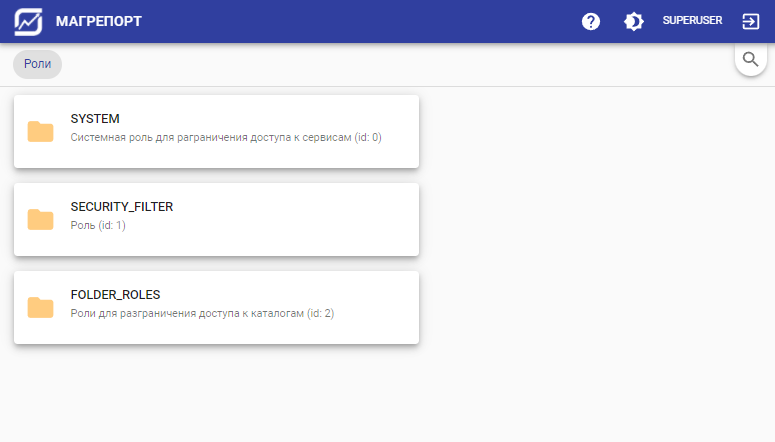
\includegraphics[width=\graphicswidth]{img/01-roles-folders.png}
		\caption{Типы ролей}
		\label{fig:roles-folders}
	\end{figure}

	В подразделе <<Роли>> пользователь не может создавать свои каталоги. Пользователь может создавать роли в каталогах FOLDER\_ROLES и SECURITY\_FILTERS, но не может создавать роли в каталоге SYSTEM. Для создания новой роли, как и для создания любых других объектов, нужно нажать на кнопку в виде знака <<+>> в правом нижнем углу экрана и выбрать единственный пункт всплывающего меню <<Добавить роль>>. При создании роли указываются её название и описание (см. рис. \ref{fig:create-role}), другие разделы редактора роли при создании недоступны - они доступны только при редактировании роли.
	
	
	\begin{figure}[h]
		\centering
		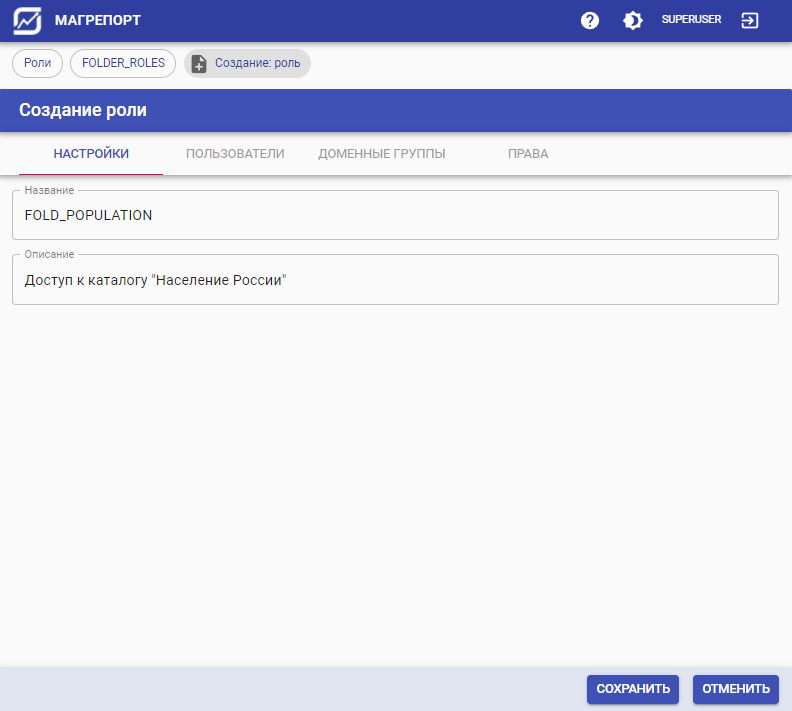
\includegraphics[width=\graphicswidth]{img/02-create-role.png}
		\caption{Создание роли}
		\label{fig:create-role}
	\end{figure}

	Для редактирования роли необходимо нажать кнопку <<Редактировать>> в левом нижнем углу карточки роли. При редактировании роли можно изменить её название, описание, а также назначить эту роль на пользователей и на доменные группы --- для этого нужно на соответствующих вкладках <<Пользователи>> и <<Доменные группы>> в строке поиска найти соответствующего пользователя или доменную группы и нажать кнопку <<Добавить>> (см. рис. \ref{fig:edit-role}). В списке пользователей, обладающих данной ролью, присутствуют как пользователи, которым непосредственно предоставлена данная роль, так и пользователи, получившие роль через доменную группу. Роль через доменную группу пользователь получает в момент входа в систему. Чтобы обновились привязки при обновлении состава доменных групп пользователя, пользователю необходимо перелогиниться в системе. Кроме того в редакторе роли на вкладке <<Права>> можно управлять правами доступа к каталогам различных объектов системы Магрепорт обладателям данной роли --- для этого нужно в поле <<Объекты>> выбрать нужный тип объекта, нажать справа от этого поля одну из кнопок <<Выдать права на чтение>> или <<Выдать права на запись>>, зайти в нужный каталог и нажать кнопку <<Выбрать>> (см. рис. \ref{fig:edit-role-folder-rights}). Измение уровня доступа --- только на чтение или на чтение и запись может быть осуществлено через флаг <<RW>> справа от каталога, на который выданы права. Другой способ выдачи прав на каталоги рассмотрен в разделе \ref{administration:folders-rights-settings}. Назначение роли на пользователей и доменные группы и измение прав на каталоги в редакторе роли происходит сразу после выбора и не требует последующего сохранения объекта.
	
	\begin{figure}[h]
		\centering
		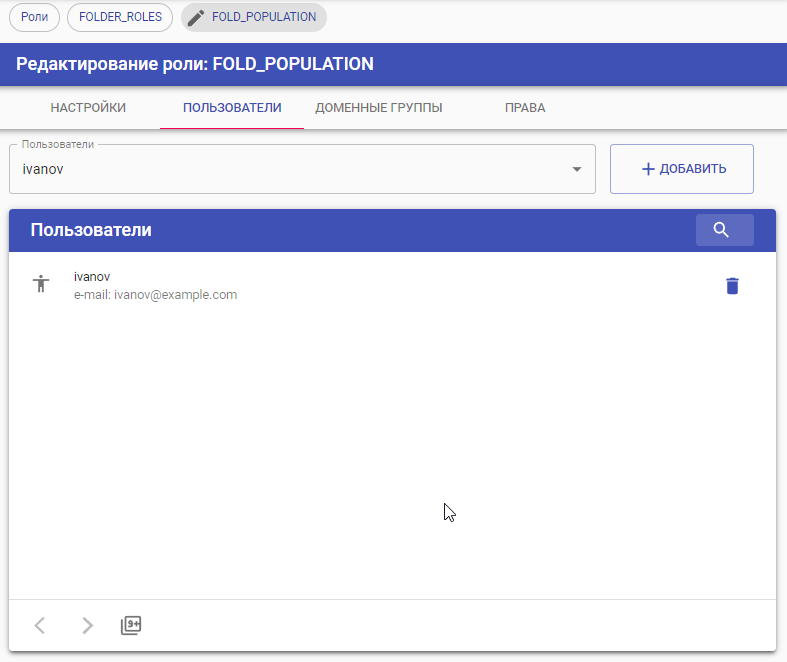
\includegraphics[width=\graphicswidth]{img/03-edit-role.png}
		\caption{Редактирование роли}
		\label{fig:edit-role}
	\end{figure}	

	\begin{figure}[h]
		\centering
		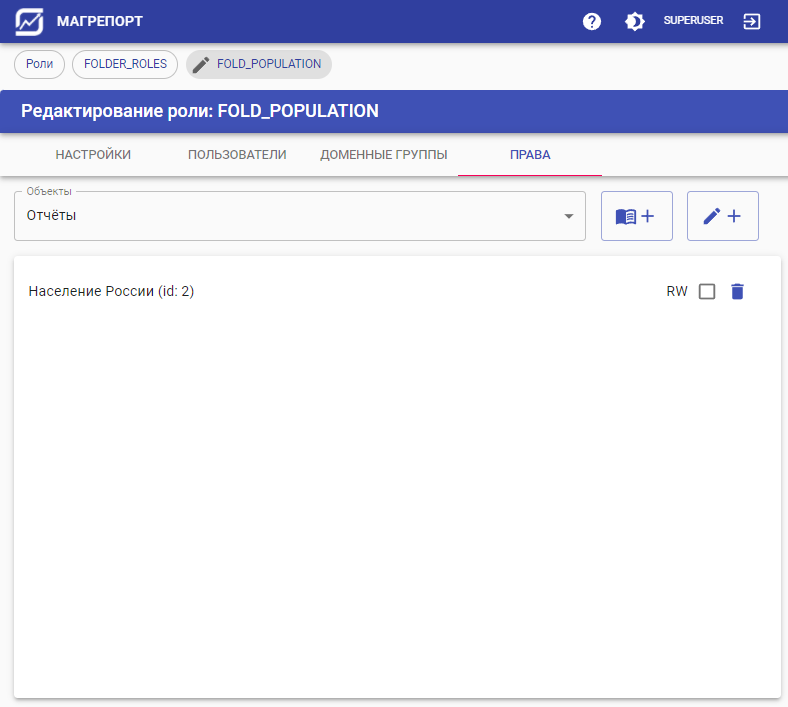
\includegraphics[width=\graphicswidth]{img/04-edit-role-folder-rights.png}
		\caption{Выдача прав на каталог роли}
		\label{fig:edit-role-folder-rights}
	\end{figure}

	При нажатии на карточку роли запускается мастер просмотра роли --- доступна вся информация о роли в режиме чтения. При нажатии на кнопку <<Редактировать>> из мастера просмотра роли можно перейти в редактор роли.
		
	\section{Управление правами пользователей}
	
	Управление правами пользователей осуществляется в подразделе <<Пользователи>> раздела <<Администрирование>> бокового меню через назначение ролей пользователям (см. рис. \ref{fig:users}).
	
	\begin{figure}[h]
		\centering
		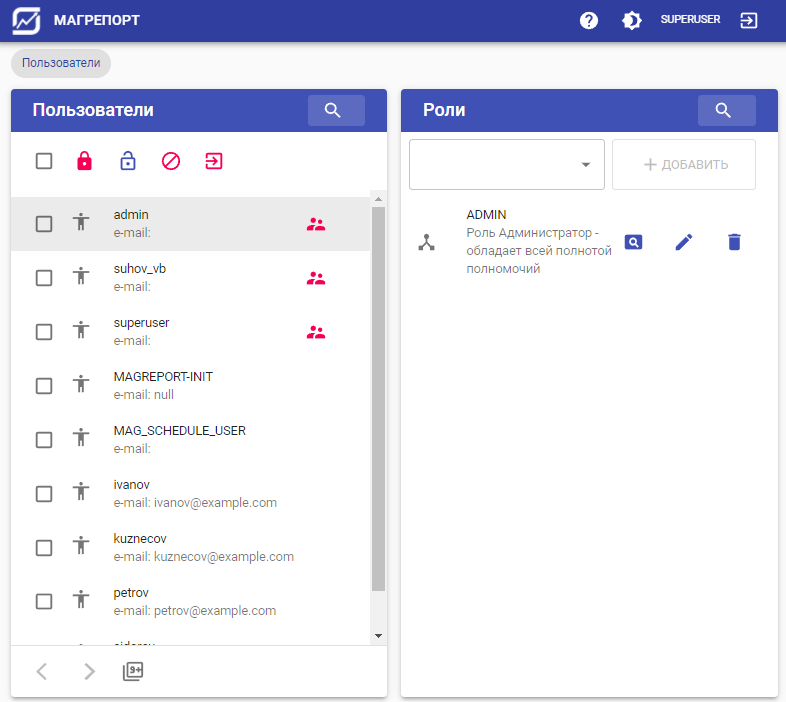
\includegraphics[width=\graphicswidth]{img/05-users.png}
		\caption{Управление ролями пользователей}
		\label{fig:users}
	\end{figure}

	Чтобы управлять набором ролей данного пользователя, необходимо выбрать этого пользователя в левой панели <<Пользователи>> (можно воспользоваться строкой поиска по логину) и в правой панели <<Роли>>, воспользовавшись поиском в строке поиска ролей, выбрать нужную роль и добавить её пользователю при помощи кнопки <<Добавить>>. Также воспользовавшись кнопкой удаления (в виде контейнера для мусора) можно снять роль с пользователя. В списке ролей пользователя показаны как роли, ваданные пользователю вручную или механизмом ASM, так и роли, полученные пользователем через доменные группы.
	
	Также в панели <<Пользователи>> есть дополнительный функционал, доступный посредством кнопок в верхней части панели:
	
	\begin{itemize}
		\item Кнопка \textit{LOCK} --- заблокировать отмеченных пользователей: переводит отмеченных галочками пользователей в статус заблокированных --- такие пользователи не могут логиниться в систему.
		
		\item Кнопка \textit{UNLOCK} --- разблокировать отмеченных пользователей: снимает блокировку с отмеченных пользователей.
		
		\item Кнопка \textit{LOGOFF} --- завершить сессию (разлогинить) выбранного пользователя (пользователя, на котором находится курсор в списке).
		
		\item Кнопка \textit{LOGOFF ALL} --- завершить сессии всех пользователей. Данная функция полезна при установке обновлений --- после обновления стоит разлогинить всех пользователей, чтобы они заново загрузили обновлённый фронтенд.
		
	\end{itemize}
	
	\section{Управление правами доступа к каталогам}\label{administration:folders-rights-settings}
	
	Правами доступа на каталоги можно управлять из редактора роли и из редактора прав каталога. Первый способ был рассмотрен ранее в разделе \ref{administration:user-roles}, второй способ будет рассмотрен в данном разделе.
	
	Права настройки прав доступа на каталоги есть только у пользователей с системной ролью ADMIN. Для входа в редактор прав каталога нужно нажать на кнопку в виде трёх вертикальных точек справа на карточке каталога (см. рис. \ref{fig:folder-rights-buttons}) и выбрать пункт выпадающего меню <<Выдать права>>.
	
	\begin{figure}[h]
		\centering
		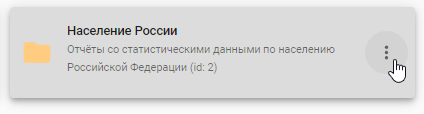
\includegraphics[width=\graphicswidth]{img/06-folder-rights-button.png}
		\caption{Кнопка входа в редактор прав каталога}
		\label{fig:folder-rights-buttons}
	\end{figure}

	В появившемся редакторе прав каталога (см. рис. \ref{fig:folder-rights-editor}) необходимо настроить права на данный каталог. Для предоставления прав на чтение каталога конкретной роли, эту роль нужно найти при помощи поиска по названию в строке поиска и нажать кнопку <<Добавить>>. В списке ролей, имеющих доступ к данному каталогу можно управлять уровнем доступа для каждой роли при помощи флага RW --- установленный флаг означает права на чтение и запись, снятый --- только на чтение (см. рис. \ref{fig:folder-rights-editor}). Если пользователь имеет несколько разных групп, на которые выданы права на каталог, то он получает максимальные права по всем этим группам --- то есть если у всех групп права только на чтение, он получает права на чтение, если хотя бы у одной группы права на чтение и запись --- он получает права на запись.
	
	\begin{figure}[h]
		\centering
		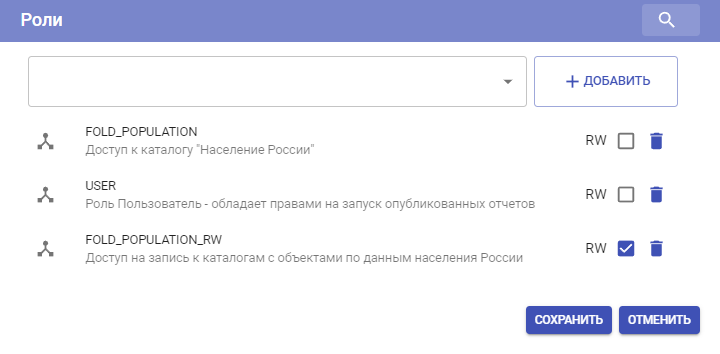
\includegraphics[width=\graphicswidth]{img/07-folder-rights-editor.png}
		\caption{Редактор прав каталога}
		\label{fig:folder-rights-editor}
	\end{figure}

	Права на запись дают возможность создания объектов в каталоге: объектов данного типа и дочерних каталогов, а также возможность копирования и переноса объектов в данный каталог. Права на чтение дают возможность просмотра содержимого каталога и содержащихся в ним объектов. Права на чтение на каталоги с отчётами дают возможность запуска отчётов, содержащихся непосредственно в данном каталоге.
	
	Права дочерних каталогов независимы от прав родительских каталогов, но при создании дочернего каталога права родительского каталога копируются в права дочернего каталога. Впоследствии права дочернего каталога могут быть изменены.
	
	\section{Просмотр заданий пользователей}
	
	В подразделе <<Задания пользователей>> администратор может увидеть задания всех пользователей системы (см. рис. \ref{fig:user-jobs}) в течение их периода хранения (см. пункт \ref{subsection:folders-settings}). Также администратор может отменить выполняющееся задание через кнопку <<Отменить>>, открыть мастер запуска отчёта с теми же значениями параметров, с которыми был запущен отчёт при помощи кнопки <<Запустить отчёт заново>> и просмотреть SQL-код запроса к БД для данного задания при помощи кнопки <<Показать SQL запрос>> (см. рис. \ref{fig:user-job-card}).
	
	\begin{figure}[h]
		\centering
		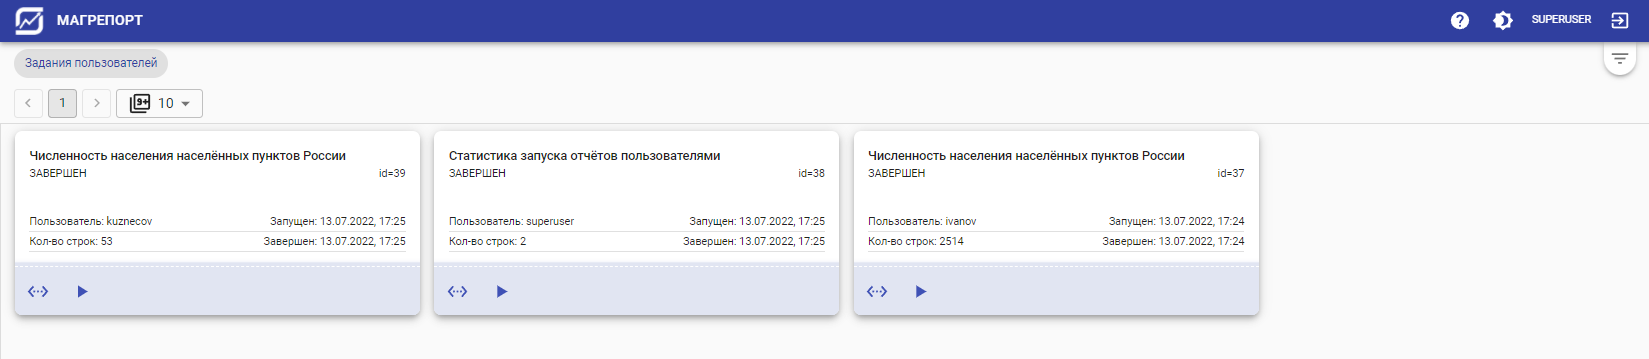
\includegraphics[width=\graphicswidth]{img/08-user-jobs.png}
		\caption{Просмотр заданий пользователей}
		\label{fig:user-jobs}
	\end{figure}
	
	
	\begin{figure}[h]
		\centering
		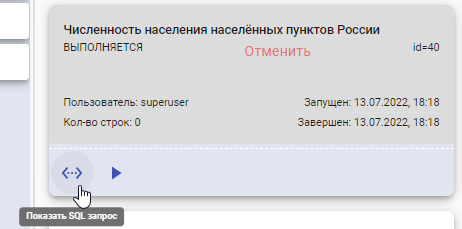
\includegraphics[width=\graphicswidth]{img/09-user-job-card.png}
		\caption{Карточка задания}
		\label{fig:user-job-card}
	\end{figure}

	При помощи кнопки <<Фильтры>> панели заданий пользователей можно открыть панель фильтрации и задать фильтрацию заданий по времени запуска, логину пользователя и статусу выполнения задания (см. рис. \ref{fig:user-job-filter}).
	
	\begin{figure}[h]
		\centering
		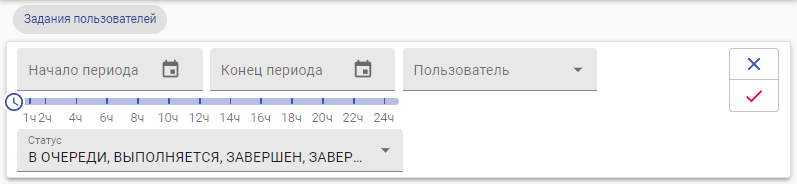
\includegraphics[width=\graphicswidth]{img/10-user-job-filter.png}
		\caption{Панель фильтрации списка заданий пользователей}
		\label{fig:user-job-filter}
	\end{figure}	

	Список заданий и их статусы не обновляются автоматически --- для обновления нужно нажать кнопку обновления в правом нижнем углу панели заданий пользователей.

	\section{Фильтры безопасности}\label{administration:security-filters}
	
	Фильтры безопасности в Магрепорте реализуют разграничение прав пользователей на уровне данных. Действие фильтров безопасности проявляется в добавлении дополнительного условия фильтрации в запрос к БД при выгрузке данных отчёта и получении значений справочников. Управление фильтрами безопасности осуществляется администраторами системы в подразделе <<Фильтры безопасности>> раздела <<Администрирование>> бокового меню.
	
	\begin{figure}[h]
		\centering
		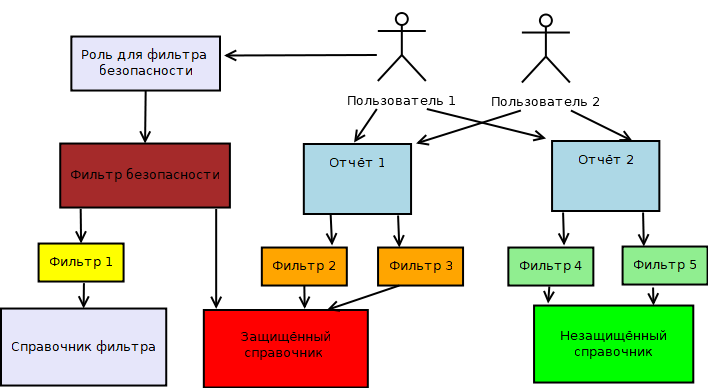
\includegraphics[width=\graphicswidth]{img/11-sf-concept-diagram.png}
		\caption{Схема действия фильтров безопасности}
		\label{fig:sf-concept-diagram}
	\end{figure}

	На рис. \ref{fig:sf-concept-diagram} представлена схема действия фильтров безопасности. На данном примере концепция фильтров безопасности может быть описана следующим образом:
	
	\begin{itemize}
		\item Фильтр безопасности привязывается к ролям и через них оказывает своё действие на пользователей, наделённых этой ролью. В рассматриваемом на схеме примере Пользователь 1 имеет привязку к фильтру безопасности, Пользователь 2 не имеет привязки к фильтру безопасности и, таким образом, не ограничен им. При привязке роли к фильтру безопасности задаётся конкретное значение ограничения, накладываемого данным фильтром безопасности (например, <<регион Москва>>).
		
		\item Фильтр безопасности строится на основе некоторого фильтра. Из данного фильтра фильтр безопасности получает набор полей (все поля фильтра с типом ID). Также этот фильтр используется при запросе значений справочника при установке ограничений фильтра безопасности для данной роли безопасности. На схеме этот фильтр обозначен как <<Фильтр 1>>, набор данных, на котором он строится --- <<Справочник фильтра>>. \textit{Фильтр безопасности автоматически не распространяет своё действие на набор данных, на котором основан фильтр, на котором строится фильтр безопасности}. Чтобы этот набор данных стал защищённым, действие фильтра безопасности нужно на него распространить явно (см. далее).
		
		\item Фильтр безопасности защищает наборы данных, на который распространено его действие. Эти наборы данных указываются явно при задании свойств фильтра безопасности. Они должны содержать набор полей фильтра безопасности (который получен из фильтра, на котором строится фильтр безопасности) --- при привязке набора данных к фильтру безопасности устанавливается соответствие полей набора данных и полей фильтра безопасности. Защита набора данных фильтром безопасности заключается в следующем:
			\begin{itemize}
				\item При любом обращении пользователя к защищённому набору данных (как через фильтры, так и через выполнение отчёта на этом наборе данных), к которому привязана роль, на которую наложены ограничения данным фильтром безопасности,  в предикат запроса (через логическое И) добавляется условие, соответствующее значению этого ограничения (например, <<region\_code = 77>>). Таким образом в фильтрах, строящихся на защищённых справочниках, пользователь просто не может выбрать недоступные ему значения, а в отчётах, строящихся на защищённых наборах данных, пользователь будет получать результат, ограниченный его ограничениями в фильтре безопасности, что бы он ни выбирал в фильтрах.
				
				\item При любом выполнении отчёта, в который добавлен фильтр, основанный на защищённом справочнике, в предикат запроса также добавляется условие, соответствующее ограничению наложенному на пользователя через роль, привязанную к фильтру безопасности. Это условие добавляется, даже если на набор данных, на котором строится отчёт, не было распространено действие фильтра безопасности и даже если пользователь ничего не выбрал в защищённом фильтре. Это позволяет, во-первых, развязать зоны ответственности админстратора и разработчика отчётов, поскольку управление ролями и фильтрами безопасности --- зона ответственности первого, а во-вторых, упростить управление правами, сконцентрировав задачу управления фильтрами безопасности на вопросе распространения их действия на справочники, на которых строятся фильтры. Если стоит задача защитить отчёт, на котором не требуется задание пользователем значения защищённого фильтра, то этот защищённый фильтр можно добавить в отчёт в виде скрытого фильтра --- таким образом он не будет выведен пользователю и при этом распространить своё действие на отчёт, тем самым <<защитив>> его.
				
			\end{itemize}
		
			На приведённой схеме защищённый набор данных обозначен как <<Защищённый справочник>>. Фильтры с номерами 2 и 3, основанные на этом наборе данных, также являются защищёнными. При этом наборы полей этих фильтров не обязаны совпадать с набором полей фильтра 1, на котором основан фильтр безопасности.
			
			\item Пользователь, обладающий ролью, привязанной к фильтру безопасности, получает ограничения, накладываемые этим фильтром безопасности при выполнении запросов от фильтров и при формировании отчёта. На схеме пользователь 1 при использовании отчёта 1 ограничен наложенными на него ограничениями фильтра безопасности через обозначенную на схеме роль для фильтра безопасности. При обращении к отчёту 2 пользователь 1 не ограничен, так как в отчёте 2 нет фильтров, защищённых данным фильтром безопасности (и сам набор данных отчёта предполагается не ограниченным этим фильтром безопасности, хоть это и не обозначено на схеме --- концепция фильтров безопасности ориентирована на ограничение именно справочников и основанных на них фильтрах, при правильном использовании этого подхода в ограничении наборов данных, на которых строятся отчёты, нет нужды). Пользователь 2 не ограничен ни при выполнении отчёта 1 (так как не обладает ролью, привязанной к фильтру безопасности), ни тем более при выполнении отчёта 2.
		
	\end{itemize}

	Для создания фильтра безопасности и управления его действием необходимо выполнить следующие шаги:
	
	\begin{itemize}
		
		\item Создать роли для фильтра безопасности --- рекомендуется создавать роли типа SECURITY\_FILTER, хоть это и не является техническим ограничением. Роли должны соответсвовать вариантам ограничений (для удобства поиска этих ролей рекомендуется давать их названиям общий префикс, например, <<SF\_>>) --- например, роль для каждого региона, по которому могут быть ограничены пользователи. Если роли и их привязки к пользователям предполагается создавать и задавать через механизм ASM (см. раздел \ref{administration:ASM}), то этот шаг создания ролей вручную пропускается.
		
		\item Создать фильтр безопасности --- эта операция выполняется через подраздел <<Фильтры безопасности>> раздела <<Администрирование>> бокового меню. Для этого, как и для всех объектов Магрепорта, необходимо создать систему каталогов и создать в них объекты <<Фильтры безопасности>> через кнопку <<плюс>> в правом нижнем углу экрана. При создании фильтра безопасности указывается его название, описание и фильтр, на котором он основан (см. рис. \ref{fig:sf-create}).
		
		\item Распространить действие фильтра безопасности на наборы данных путём нажатия кнопки <<плюс>> на закладке <<Наборы данных>> мастера создания фильтра безопасности, выбора набора данных и указания соответствия полей фильтра и набора данных (см. рис. \ref{fig:bind-sf-to-dataset}).
		
		\item Задать ограничения фильтра безопасности для каждой роли, на которую распространяется действие фильтра. Это делается на вкладке <<Привязка роли>> мастера создания фильтра безопасности (см. рис. \ref{fig:sf-bind-to-role}).
		
	\end{itemize}

	\begin{figure}[h]
		\centering
		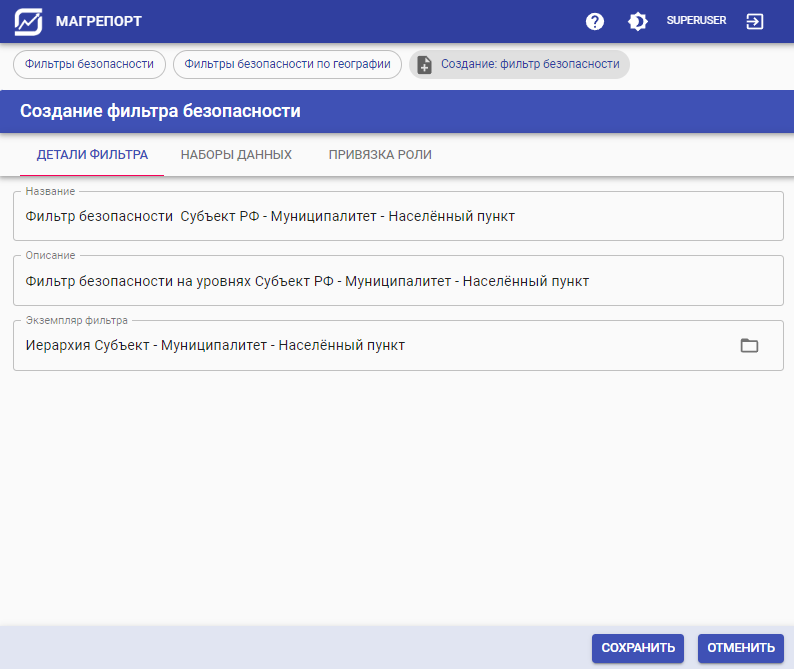
\includegraphics[width=\graphicswidth]{img/12-sf-create.png}
		\caption{Создание фильтра безопасности}
		\label{fig:sf-create}
	\end{figure}

	\begin{figure}[h]
		\centering
		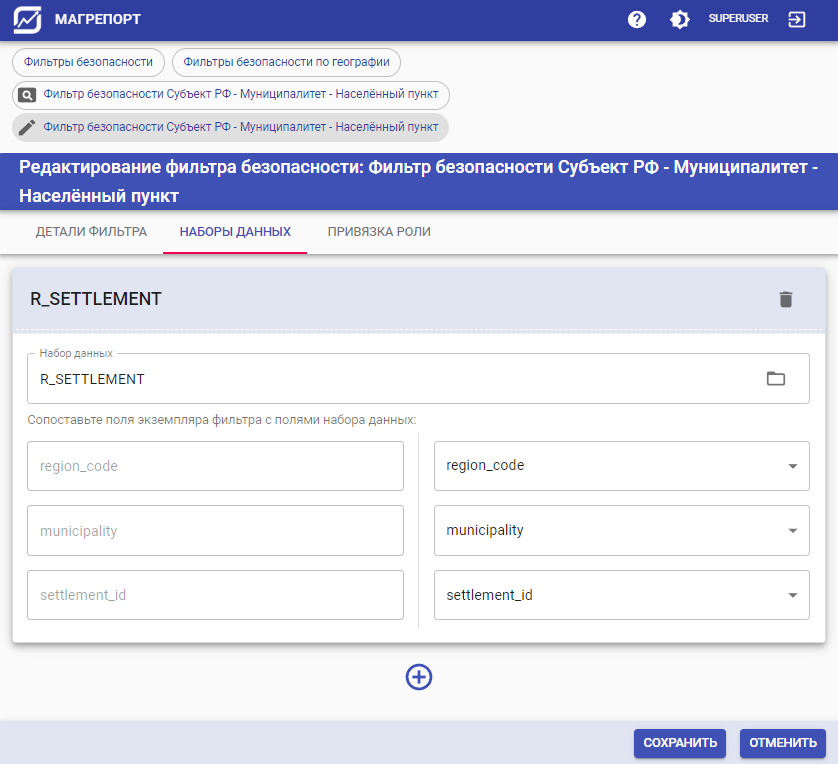
\includegraphics[width=\graphicswidth]{img/13-bind-sf-to-dataset.png}
		\caption{Распространение действия фильтра безопасности на набор данных}
		\label{fig:bind-sf-to-dataset}
	\end{figure}

	\begin{figure}[h]
		\centering
		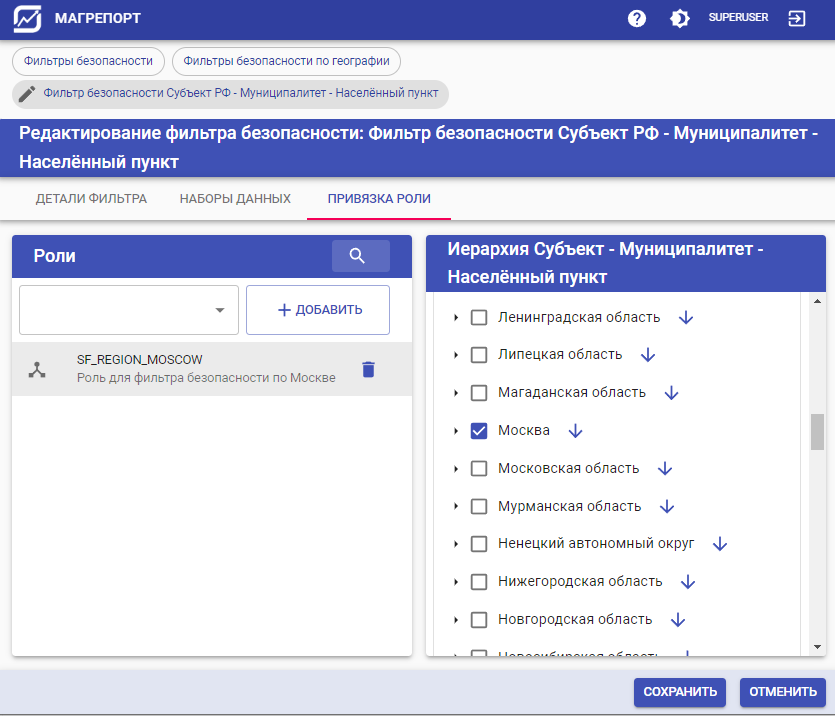
\includegraphics[width=\graphicswidth]{img/15-sf-bind-to-role.png}
		\caption{Задание ограничений фильтра безопасности для роли}
		\label{fig:sf-bind-to-role}
	\end{figure}

	При запуске отчёта пользователем, ограниченым фильтром безопасности через назначенную пользователю роль, привязанную к фильтру безопасности, пользователь ограничен в выборе возможных значений в фильтре (см. рис. \ref{fig:sf-action}). Кроме того, даже если пользователь не сделает никакого выбора в фильтре, результат выполнения отчёта всё равно будет ограничен наложенным через фильтр безопаности условием (см. рис. \ref{fig:sf-report-result}).

	\begin{figure}[h]
		\centering
		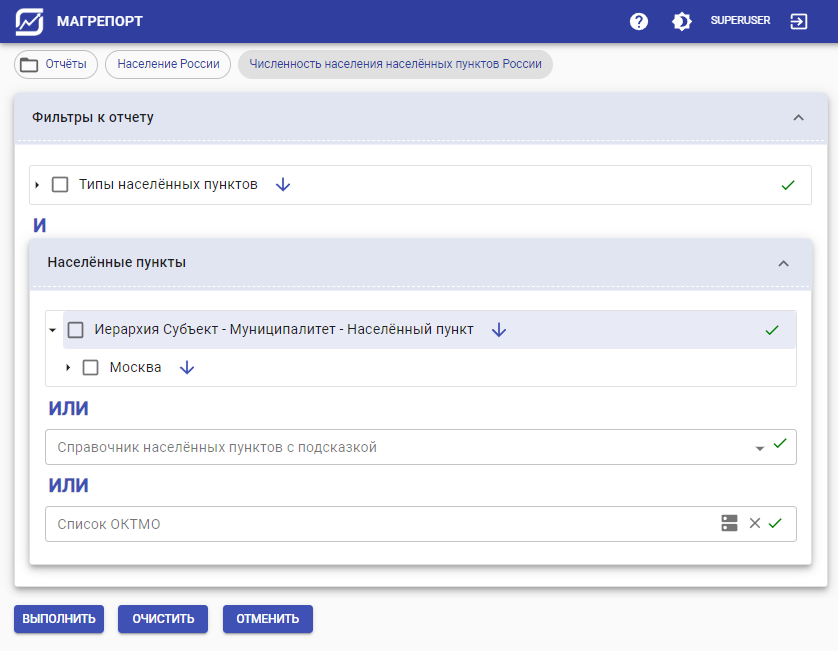
\includegraphics[width=\graphicswidth]{img/14-sf-action.png}
		\caption{Действие фильтра безопасности}
		\label{fig:sf-action}
	\end{figure}

	\begin{figure}[h]
		\centering
		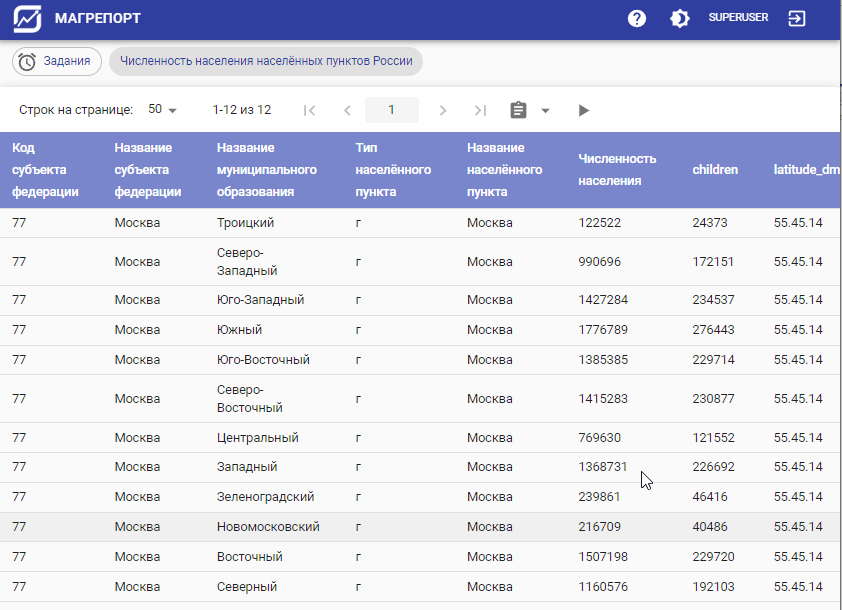
\includegraphics[width=\graphicswidth]{img/16-sf-report-result.png}
		\caption{Результат выполнения отчёта при условии действия фильтра безопасности}
		\label{fig:sf-report-result}
	\end{figure}
	
	\begin{NB}
		Не имеет смысла на одного и того же пользователя накладывать несколько ролей, привязанных к одному и тому же фильтру безопасности, со взаимоисключающими ограничениями (например, <<регион Москва>> и <<регион Санкт-Петербург>>) --- это приведёт к тому, что пользователь не получит никаких данных, поскольку фильтры безопасности объединяются между собой через логическое И. Если требуется пользователю задать комлексное ограничение, соответствующее объединению нескольких элементарных ограничений, для которых созданы универсальные роли фильтров безопасности, то для такого пользователя необходимо создать индивидуальную роль, на которую наложены соответствующие ограничения. Удобнее это делать через механизм ASM (см. раздел \ref{administration:ASM}).
	\end{NB}
	
	\section{Администрирование объектов ASM}\label{administration:ASM}
	
	В результате эволюции продукта так сложилось, что механизм автоматического управления безопасностью имеет в названии англоязычный акроним ASM, что означает \textit{Automated Security Management}. Данный функционал предназначен для:
	\begin{itemize}
		\item автоматического создания ролей безопасности;
		\item автоматического управления привязкой ролей к пользователям;
		\item автоматического управления привязкой ролей к фильтрам безопасности и задания ограничений данного фильтра безопасности для данной роли.
	\end{itemize}
	Данные для создания ролей и привязок и задания ограничений ASM берёт из БД.
	
	Настройка и действие механизма ASM будут рассмотрены на примере объектов, созданных в главе \ref{chapter:developing}, и фильтра безопасности, изображенного на рисунках \ref{fig:sf-create}, \ref{fig:bind-sf-to-dataset}, предназначенного для ограничений пользователей по географическим объектам.
	
	Под объектом ASM здесь и далее понимается объект в системе Магрепорт, хранящий информацию об объектах БД, предоставляющих данные о ролях, привязках и ограничениях, и о фильтре безопаности, используемом для наложения ограничений. Управление объектами ASM осуществляется в подразделе <<Управление ASM>> раздела <<Администрирование>> бокового меню. 
	
	Для создания и работы объекта ASM требуются следующие три таблицы (или представления) в БД (под CDC-таблицей понимается таблица или представление, запрос к которой возвращает изменения по сравнению с предыдущей загрузкой данных --- от англ. \textit{Change Data Capture} --- захват изменений данных):
	\begin{itemize}
		\item CDC-таблица для ролей, условно называемая \textit{GROUP\_SOURCE}. Эта таблица должна содержать информацию о новых и удаляемых ролях. Структура таблицы должна быть следующей:
	
		\begin{center}
			\begin{tabular}{|l|p{0.5\textwidth}|}
				\hline
				Название поля & Содержание поля \\
				\hline
				CHANGE\_TYPE & Текстовое поле со значением: \newline 
				'I' --- если роль должна быть добавлена, 'D' --- если роль должна быть удалена \\
				\hline
				ROLE\_NAME & Текстовое поле с названием добавляемой или удаляемой роли \\
				\hline
			\end{tabular}
		\end{center}
	
		\item CDC-таблица для привязок пользователей к ролям, условно называемая \textit{USER\_MAP\_SOURCE}. Эта таблица должна содержать информацию о новых и удаляемых привязках. Структура таблицы должна быть следующей:
		
		\begin{center}
			\begin{tabular}{|l|p{0.5\textwidth}|}
				\hline
				Название поля & Содержание поля \\
				\hline
				CHANGE\_TYPE & Текстовое поле со значением: \newline 
				'I' --- если роль должна быть добавлена, 'D' --- если роль должна быть удалена \\
				\hline
				ROLE\_NAME & Текстовое поле с названием добавляемой или удаляемой роли \\
				\hline
				USER\_NAME & Логин пользователя, которому добавляется или у которого удаляется роль \\
				\hline
			\end{tabular}
		\end{center}		
	
		\item Таблица с ограничениями ролей для данного фильтра безопасности, условно называемая\\ \textit{PERMISION\_SOURCE}. Эта таблица содежит информацию об ограничениях, накладываемых на роль. Таблица должна иметь следующую структуру:
		
		\begin{center}
			\begin{tabular}{|l|p{0.5\textwidth}|}
				\hline
				Название поля & Содержание поля \\
				\hline
				CHANGE\_TYPE & Текстовое поле со значением 'I': все ограничения для данной роли всегда перезаписываются заново \\
				\hline
				ROLE\_NAME & Текстовое поле с названием роли, для которой устанавливаются ограничения \\
				\hline
				поля с ключами сущностей & иерахическая структура полей со значениями ключей, соответствующих данному ограничению. Если уровней больше одного, то ограничения могут бытьь заданы только для первых нескольких уровней, в этом случае для нижележащих уровыней должны быть заданы значения null (см. пример ниже) \\
				\hline
			\end{tabular}
		\end{center}		
		
	\end{itemize}
	
	В рассматриваемом примере в качестве GROUP\_SOURCE выступает представление \\ V\_ASM\_GEO\_ROLE\_CDC, содержащее следующие данные:
		\begin{center}
			\begin{tabular}{|l|l|}
				\hline
				\textbf{CHANGE\_TYPE} & \textbf{ROLE\_NAME} \\
				\hline
				'I' & 'SF\_GEO\_IVANOV'\\
				\hline
			\end{tabular}
		\end{center}
	Это означает, что должна быть создана роль \textit{SF\_GEO\_IVANOV}.
	
	\begin{adminnote}
		Удобной практикой является создание индивидуальных ролей безопасности в следующем формате: SF\_<обозначение фильтра безопасности>\_<логин пользователя>. В этом случае если на пользователя распространяется данный фильтр безопасности в результате работы ASM будет создана соответствующая роль. Впоследствии легко будет выяснить, какие ограничения наложены на конкретного пользователя.
	\end{adminnote}

	В качестве USER\_MAP\_SOURCE выступает представление V\_ASM\_GEO\_USER\_ROLE\_CDC, содержащее следующие данные:
		\begin{center}
			\begin{tabular}{|l|l|l|}
				\hline
				\textbf{CHANGE\_TYPE} & \textbf{ROLE\_NAME} & \textbf{USER\_NAME} \\
				\hline
				'I' & 'SF\_GEO\_IVANOV' & 'ivanov'\\
				\hline
			\end{tabular}
		\end{center}	
	Это означает, что роль \textit{SF\_GEO\_IVANOV} должна быть назначена пользователю \textit{ivanov}.
	
	В качестве PERMISION\_SOURCE выступает представление V\_ASM\_GEO\_ROLE\_RIGHTS, содержащее следующие данные:
		\begin{center}
		\begin{tabular}{|l|l|l|l|l|}
			\hline
			\textbf{CHANGE\_TYPE} & \textbf{ROLE\_NAME} & \textbf{region\_code} & \textbf{municipality} & \textbf{settlement\_id} \\
			\hline
			'I' & 'SF\_GEO\_IVANOV' & 23 & 'Город Краснодар' &	25233 \\
			\hline
			'I' & 'SF\_GEO\_IVANOV' & 77 & 'Центральный' &	null \\
			\hline
			'I' & 'SF\_GEO\_IVANOV' & 78 & null & null \\
			\hline
		\end{tabular}
	\end{center}
	Это означает, что роли \textit{SF\_GEO\_IVANOV} назначаются ограничения по географии: для данной роли доступны данные по хутору им. Ленина (settlement\_id = 25233) муниципального образования город Краснодар Краснодарского края, по муниципальному образованию Центральный административный округ субъекта федерации город Москва и по всему субъекту федерации город Санкт-Петербург.
	
	Данные представления необходимо добавить в Магрепорт как наборы данных (см. рис. \ref{fig:asm-cdc-datasets}).
	
	\begin{figure}[h]
		\centering
		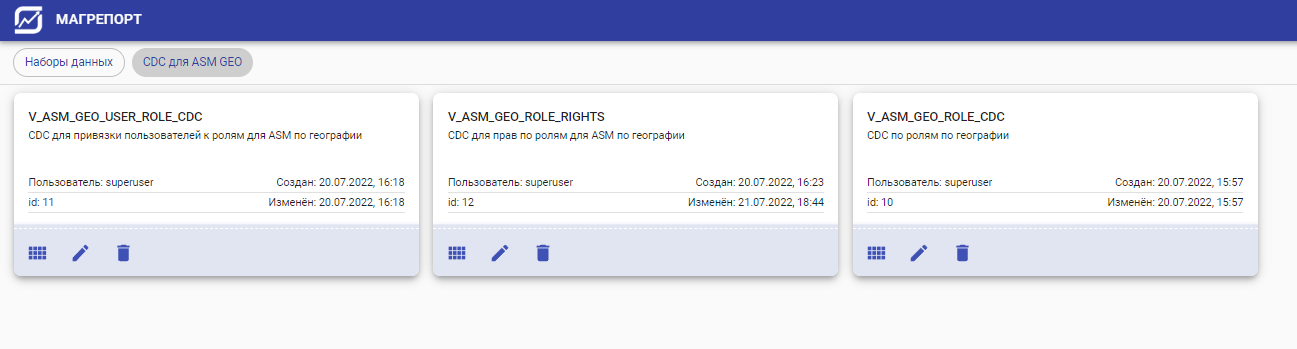
\includegraphics[width=\graphicswidth]{img/17-asm-cdc-datasets.png}
		\caption{Наборы данных для ASM}
		\label{fig:asm-cdc-datasets}
	\end{figure}

	После этого необходимо создать объект ASM (на вкладке <<Детали объекта ASM>> указывается тип ролей, которые будут создаваться данным объектом --- почти всегда это SECURITY\_FILTER, название и описание объекта), указать на соответствующих вкладках созданные наборы данных и привязать фильтр безопасности (см. рис. \ref{fig:asm-details}, \ref{fig:asm-group-source}, \ref{fig:asm-user-map-source}, \ref{fig:asm-permission-source-1}, \ref{fig:asm-permission-source-2}).
	
	\begin{figure}[h]
		\centering
		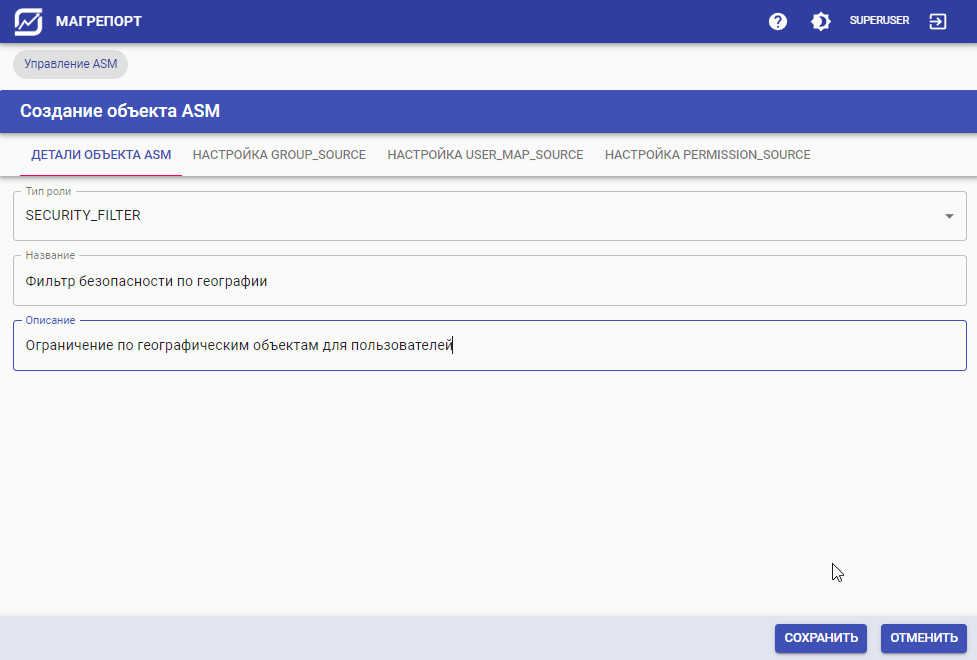
\includegraphics[width=\graphicswidth]{img/18-asm-details.png}
		\caption{Создание объекта ASM}
		\label{fig:asm-details}
	\end{figure}	
	
	\begin{figure}[h]
		\centering
		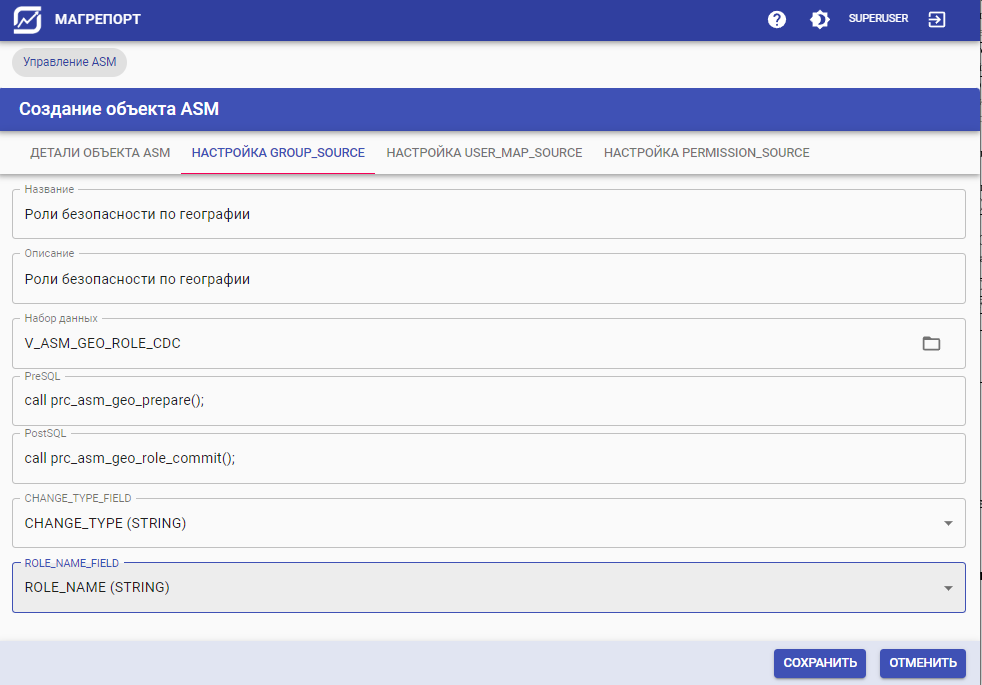
\includegraphics[width=\graphicswidth]{img/19-asm-group-source.png}
		\caption{Задание GROUP\_SOURCE для объекта ASM}
		\label{fig:asm-group-source}
	\end{figure}


	\begin{figure}[h]
		\centering
		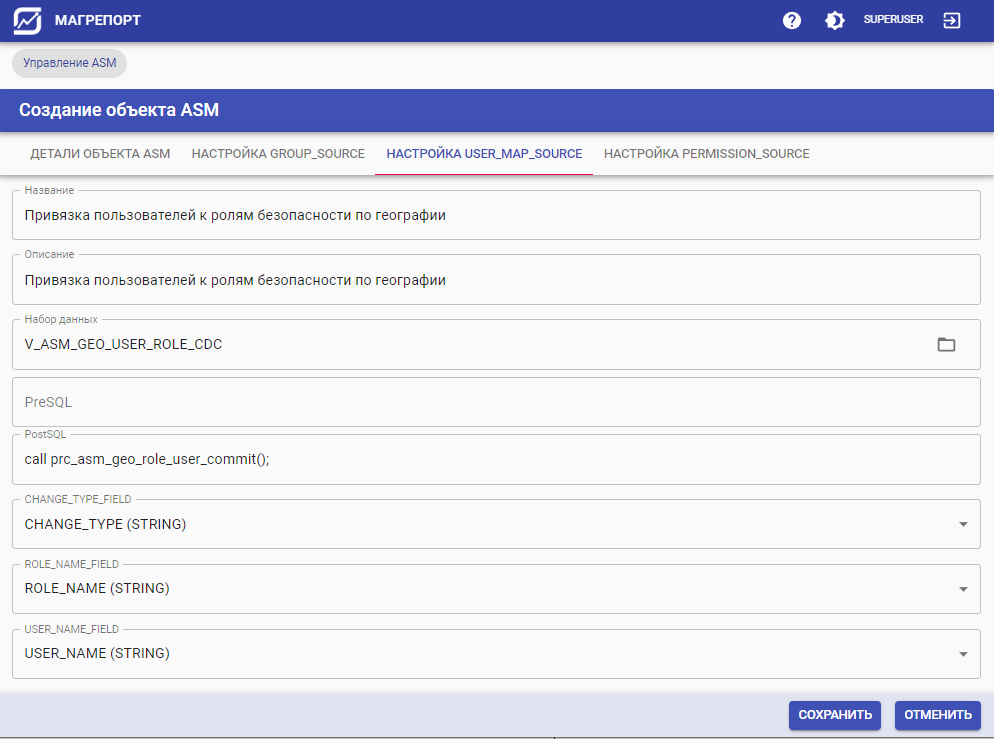
\includegraphics[width=\graphicswidth]{img/20-asm-user-map-source.png}
		\caption{Задание USER\_MAP\_SOURCE для объекта ASM}
		\label{fig:asm-user-map-source}
	\end{figure}


	\begin{figure}[h]
		\centering
		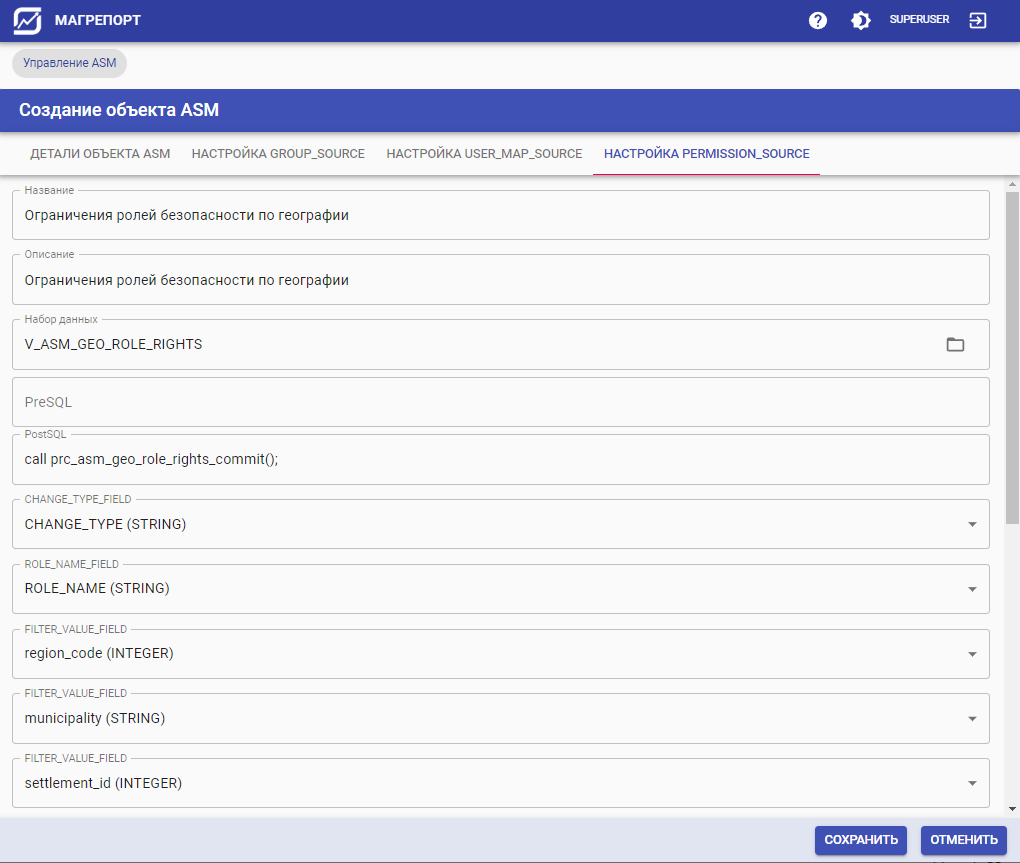
\includegraphics[width=\graphicswidth]{img/21-asm-permission-source-1.png}
		\caption{Задание PERMISSION\_SOURCE для объекта ASM}
		\label{fig:asm-permission-source-1}
	\end{figure}


	\begin{figure}[h]
		\centering
		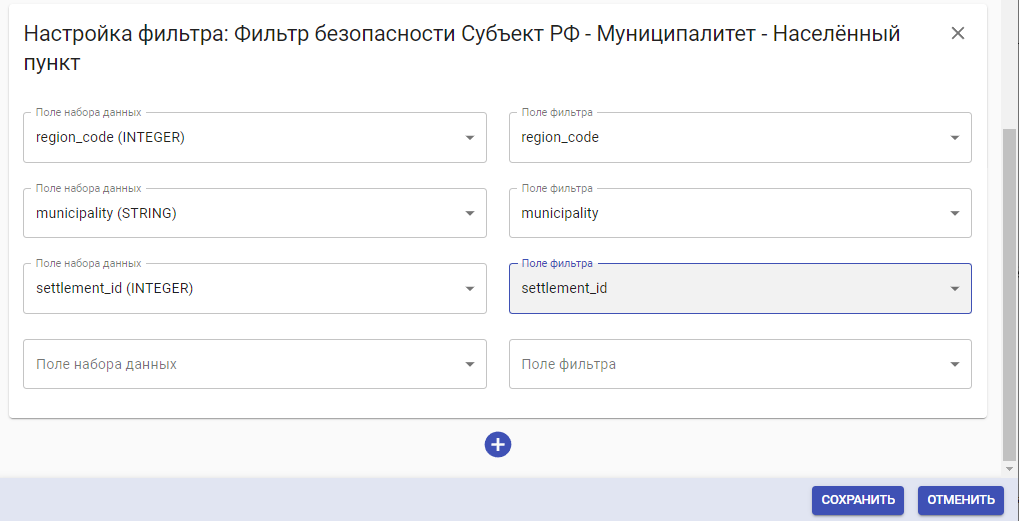
\includegraphics[width=\graphicswidth]{img/22-asm-permission-source-2.png}
		\caption{Задание фильтра безопасности для объекта ASM}
		\label{fig:asm-permission-source-2}
	\end{figure}

	Отдельно стоит остановиться на задании таблицы PERMISSION\_SOURCE и фильтра безопасности. При разметке полей таблицы PERMISSION\_SOURCE нужно в правильном порядке (в порядке иерархической подчинённости) указать все поля ключей сущностей, указываемых в таблице. После этого нужно нажать знак <<плюс>> и выбрать фильтр безопасности. После этого нужно указать соответствие полей ключей сущностей таблицы PERMISSION\_SOURCE и фильтра безопасности. Фильтров безопасности можно указать несколько (хотя трудно представить сценарий, при котором это было бы необходимо).
	
	Кроме задания наборов данных для импорта объект ASM позволяет задать SQL-запросы, выполняемые до и после каждого импорта, в полях PreSQL и PostSQL соответственно. Такими запросами могут быть вызовы процедур, подготавливающих данные в CDC-таблицах и фиксирующие факт захвата данных. Импорт данных для источников GROUP\_SOURCE, USER\_MAP\_SOURCE и PERMISSION\_SOURCE и вызов соответствующих PreSQL и PostSQL запросов производится последовательно в указанном порядке (сначала GROUP\_SOURCE, затем USER\_MAP\_SOURCE, затем PERMISSION\_SOURCE).
	
	Объекты ASM осущесвляют импорт данных в соответсвии с заданным в параметрах системы расписанием (см. пункт \ref{subsection:asm-properties}). Кроме того, можно выполнить импорт вручную: для этого нужно выделить кликом мыши несколько объектов ASM и нажать кнопку <<Обновить ASM>> в верху раздела управления ASM (см. рис. \ref{fig:asm-update}).
	
	\begin{figure}[h]
		\centering
		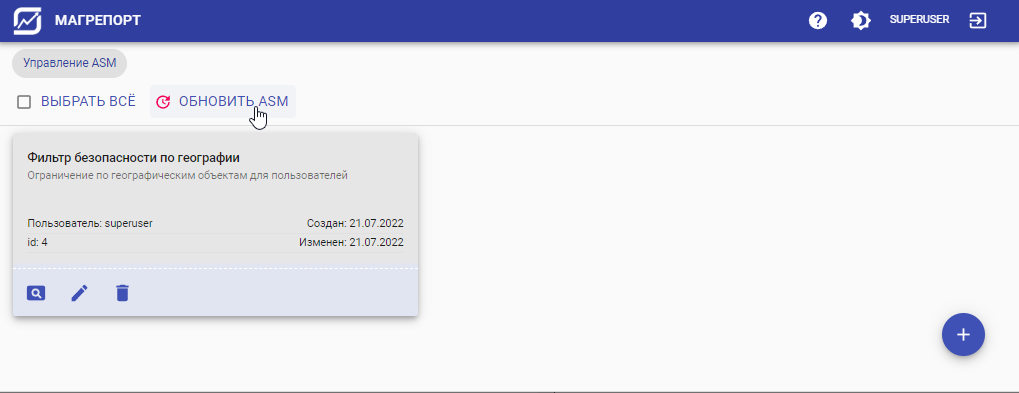
\includegraphics[width=\graphicswidth]{img/23-asm-update.png}
		\caption{Обновление объекта ASM}
		\label{fig:asm-update}
	\end{figure}	

	После выполнения импорта данных пользователь ivanov будет иметь соответствующие ограничения на получение данных (см. рис. \ref{fig:asm-role-action}).

	\begin{figure}[h]
		\centering
		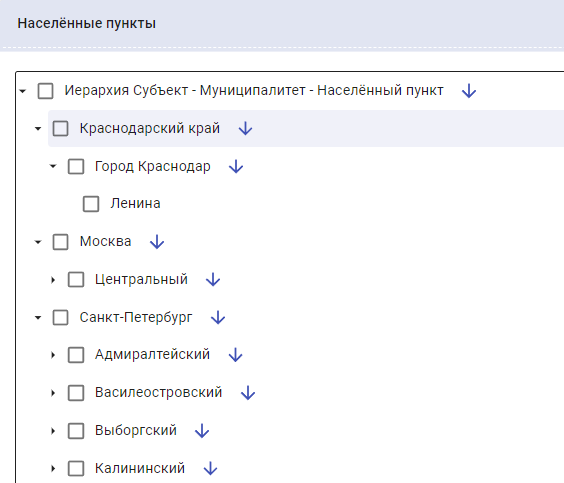
\includegraphics[width=\graphicswidth]{img/24-asm-role-action.png}
		\caption{Действие фильтра безопасности}
		\label{fig:asm-role-action}
	\end{figure}

	Выполнение импорта не приводит к сбоям в случае возможных конфликтов при импорте данных:
		\begin{itemize}
			\item Если добавляется существующая роль или существующая привязка пользователя к роли, дубли в этом случае также не создаются.
			\item Если удаляется несуществующая роль или несуществующая привязка пользователя к роли.
			\item Если добавляется привязка пользователя к несуществующей роли, в этом случае просто ничего не добавляется.
			\item Если добавляются ограничения на несуществующую роль, в этом случае просто ничего не добавляется.
			\item Если в рамках одного и того же импорта одна и та же роль или привязка идёт и с типом изменения 'D', и с типом изменения 'I' --- результат импорта будет такой, как будто она идёт только с типом изменения 'I'.
		\end{itemize}

		Описанные особенности импорта данных механизмом ASM дают простой способ создания CDC-представлений, не требующий истинной реализации механизмов захвата изменений данных. А именно: пусть имеется таблица всех пользователей \textit{USERS} с полем \textit{login}	и таблица ограничений некоторых пользователей по какой-либо сущности \textit{RESTRICTED\_USERS} с полями \textit{login} и \textit{entity\_id}, показывающая, что данный пользователь имеет права только на экземпляры данной сущности с ключами, соответствующими его логину по данной таблице, а на другие не имеет. При этом пользователи, отсутствующие в \textit{RESTRICTED\_USERS}, предполгаются имеющими права на все экземпляры данной сущности. В этом случае в качестве GROUP\_SOURCE можно использовать результат следующего запроса:

		\begin{lstlisting}[language=SQL]
	select
		'D' as CHANGE_TYPE,
		'SF_ENT_' || UPPER(login) as ROLE_NAME
	from
		USERS
	union all
	select
		MAX('I') as CHANGE_TYPE,
		'SF_ENT_' || UPPER(login) as ROLE_NAME
	from
		RESTRICTED_USERS
	group by
		login
		\end{lstlisting}

		В качестве USER\_MAP\_SOURCE:
		\begin{lstlisting}[language=SQL]
	select
		MAX('I') as CHANGE_TYPE,
		'SF_ENT_' || UPPER(login) as ROLE_NAME,
		LOWER(login) as USER_NAME
	from
		RESTRICTED_USERS
	group by
		login
	\end{lstlisting}
		И в качестве PERMISSION\_SOURCE:
		\begin{lstlisting}[language=SQL]
	select
		'I' as CHANGE_TYPE,
		'SF_ENT_' || UPPER(login) as ROLE_NAME,
		entity_id
	from
		RESTRICTED_USERS
	\end{lstlisting}		
		
		Единственная информация, которая при реализации такого способа не сохраняется --- это когда произошли те или иные изменения прав пользователя. Для сохранения этой информации можно создать дополнительные исторические таблицы и воспользоваться PreSQL и PostSQL при импорте данных объекта ASM.
		
		Однако, если списка всех пользователей в БД, предоставляющей информацию об ограничениях, нет, то для того, чтобы снимать ограничения с пользователей, на которые они ранее распространялись и перестали распространяться, придётся реализовавывать захват изменений на строне БД теми или иными методами.
	
	\section{Просмотр логов системы}
	
	Текущий файл логов Магрепорта можно скачать в подразделе <<Логи>> раздела <<Администрирование>> бокового меню. Архивные файлы логов можно получить только непосредственно из файловой системы хоста Магрепорта.
	
	\section{Системные настройки}
	
	Системные настройки находятся в подразделе <<Настройки>> раздела <<Администрирование>> бокового меню. В настоящий момент все настройки относятся к настройке почтовой системы. Их описание дано в пункте \ref{subsection:email-settings}.
	
	\section{Шаблоны текстов системеных писем}\label{section:letters-templates}
	
	Магрепорт отправляет письма в разных ситуациях: при отправке отчётов по почте, при истечении срока действия подписки, при возникновении ошибок выполнения отчёта по подписке и других. В текущией версии Магрепорта все эти ситуации относятся к функционалу выполнения отчётов по расписанию (см. раздел \ref{administration:schedule-reports}). Для каждого из этих типов писем существует шаблон, который можно отредактировать. Этот функционал доступен в каталоге SCHEDULE в подразделе <<Тексты системных писем>> раздела <<Администрирование>>. Существуют следующие шаблоны писем:
	\begin{itemize}
		\item Шаблон письма с отчётом --- такое письмо отправляется при успешном выполнении отчёта по расписанию с отправкой файла отчёта в самом письме. Настройки конретной рассылки могут перекрывать действие шаблона (см. раздел \ref{administration:schedule-reports}) --- если для конкретной рассылки заданы свои значения для темы или тела письма, они заменяют значения из шаблона.
		
		\item Шаблон письма со ссылкой на скачивание отчёта --- такое письмо отправляется при успешном выполнении отчёта по расписанию с отправкой ссылки на скачивание файла. Настройки конретной рассылки, как и в предыдущем случае, могут перекрывать действие шаблона.
		
		\item Шаблон письма с сообщением об ошибке для администраторов --- такое письмо отправляется на адрес администраторов сервера (см. пункт \ref{subsection:other-settings}) при возникновении ошибки при выполенении отчёта по расписанию.
		
		\item Шаблон письма с сообщением об ошибке для пользователей --- такое письмо отправляется на адрес получателей сообщений об ошибках при возникновении ошибки при выполенении отчёта по расписанию.		
		
		\item Шаблон письма о готовности отчета по расписанию --- такое письмо отправляется при успешном выполнении отчёта по расписанию с добавлением результата выполнения отчёта в задание пользователя (то есть без отправки файла или ссылки на скачаивание файла в письме).
		
		\item Шаблон письма об истечении срока действия рассылки --- такое письмо отправляется всем получателям рассылки, когда до истечения срока действия рассылки остаётся менее установленного временного интервала (см. пункт \ref{subsection:schedule-service-settings}).
		
		\item Шаблон письма об изменении отчета, участвующего в рассылке --- такое письмо отправляется на адрес администраторов сервера (см. пункт \ref{subsection:other-settings}) при внесении изменений в состав фильтров отчёта, если выполнение этого отчёта поставлено на расписание. При этом сама рассылка становится невалидной.
		
		\item Шаблон письма для продления действия рассылки --- такое письмо отправляется всем получателям рассылки, когда срок действия рассылки истёк.
		
		\item Добавочный текст о скором истечении срока действия рассылки --- если близится срок окончания действия подписки (см. пункт \ref{subsection:schedule-service-settings}) значение поля <<Тело письма>> шаблона добавляется в письмо с выполненным отчётом, либо ссылкой на выполненный отчёт, либо с сообщением о готовности отчёта по расписанию.
		
	\end{itemize}

	При редактировании тела письма в шаблоне применяются html-теги \textit{b, i, u, strike, sup, sub, p}. Для выделения части текста этим тегами можно воспользоваться кнопками панели инструментов, расположенными непосредственно под полем редактирования тела письма. Для этого нужно нажать соответствующую кнопку и после этого курсором мыши выделить часть текста. Поскольку к тексту письма применяется html-форматирование, переводы строк в тексте игнорируются. Чтобы разбивать текст на абзацы необходимо применять html-тег \textit{p}. Также в панели инструментов расположена кнопка предварительного просмотра (см. рис. \ref{fig:letter-template-editor}).
	
	В теле и в заголовке письма можно делать макроподстановки с различной информацией, относящимися к объекту письма. Кнопки со различными вариантам и макроподстановок расположены в панели инструментов под полем редактирования тела письма. Необходимо нажать кнопку и кликнуть мышью в поле тела или темы письма --- в этом месте будет вставлен соответствующий макрос. Если при выполнении рассылки макрос не релевантен объекту письма (например, <<текст ошибки>> не имеет значения в контексте письма с результатами выполнения отчёта, поскольку письмо с выполненным отчётом отправляется только для успешно выполненного отчёта), он заменяется пустым значением.
	
	\begin{figure}[h]
		\centering
		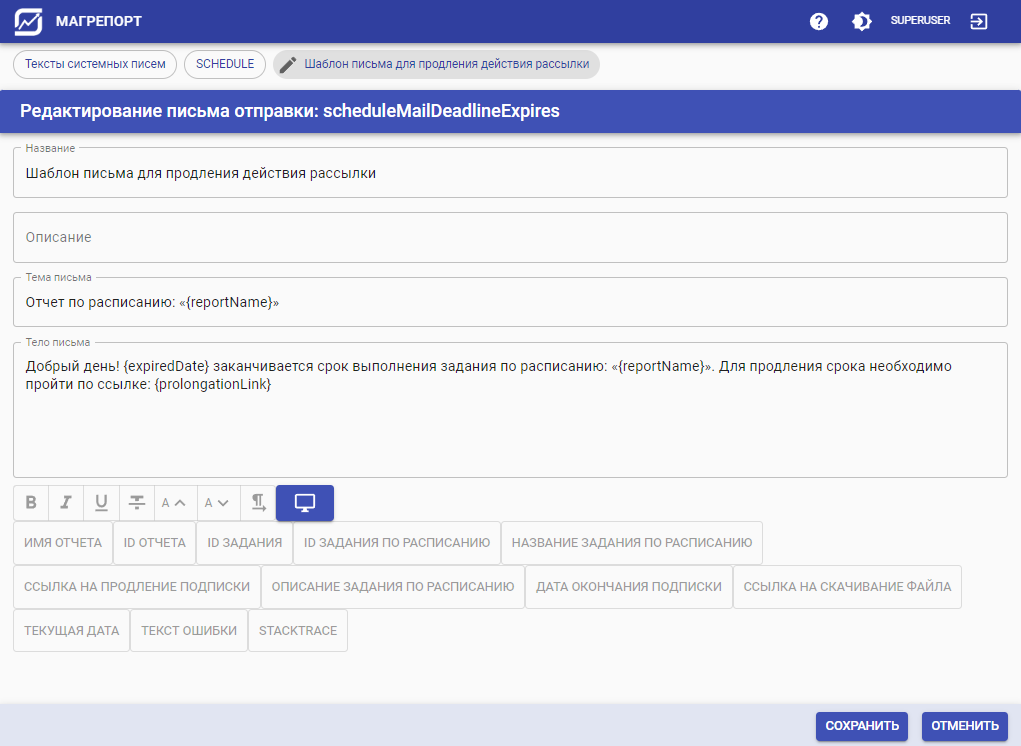
\includegraphics[width=\graphicswidth]{img/25-letter-template-editor.png}
		\caption{Редактирование шаблона письма}
		\label{fig:letter-template-editor}
	\end{figure}	
	
	\section{Отправка писем}
	
	В магрепорте предусмотрен функционал разовой отправки письма пользователям системы. Для этого необходимо воспользоваться формой в подразделе <<Рассылка писем>>. Через данную форму можно отправить письма только пользователям системы Магрепорт и только тем из них, у которых заполнено значение адреса электронной почты (импортируется из LDAP).
	
	Для этого в форме необходимо кликнуть на одно из полей указания адресата (<<Кому>>, <<Копия>> или <<Скрытая копия>>) и в появившейся форме выбрать пользователей в качестве адресатов (см. рис. \ref{fig:send-mail-select-users}). При выборе пользователей можно использовать фильтрацию по ролям, если в графе <<Пользователи>> выбрать значение <<Роль>> и в графе <<Список ролей>> указать соответствующую роль. После этого можно добавить в адресаты некоторых или всех пользователей с данной ролью. Например, таким образом можно отправить уведомление всем пользователям, имеющим доступ к данному каталогу или всем пользователям с правами разработчика.
	
	\begin{figure}[h]
		\centering
		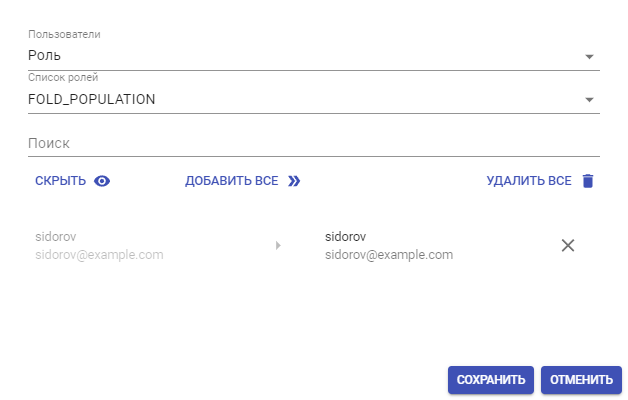
\includegraphics[width=\graphicswidth]{img/26-send-mail-select-users.png}
		\caption{Форма выбора пользователей в получатели письма}
		\label{fig:send-mail-select-users}
	\end{figure}

	Кроме заполнения списка адресатов в форме отправки письма (см. рис. \ref{fig:send-mail-form}) можно	указать тему письма и текст самого письма. В тексте письма можно использовать html-форматирование. Для тегов \textit{b, i, u, strike, sup, sub, p} предусмотрены кнопки в панели инструментов над полем текста письма. Чтобы воспользоваться кнопками, нужно нажать кнопку и выделить часть текста --- этот фрагмент будет заключён в соответствующий тег. Для разбития текста на абзацы нужно использовать тег \textit{p}.

	\begin{figure}[h]
		\centering
		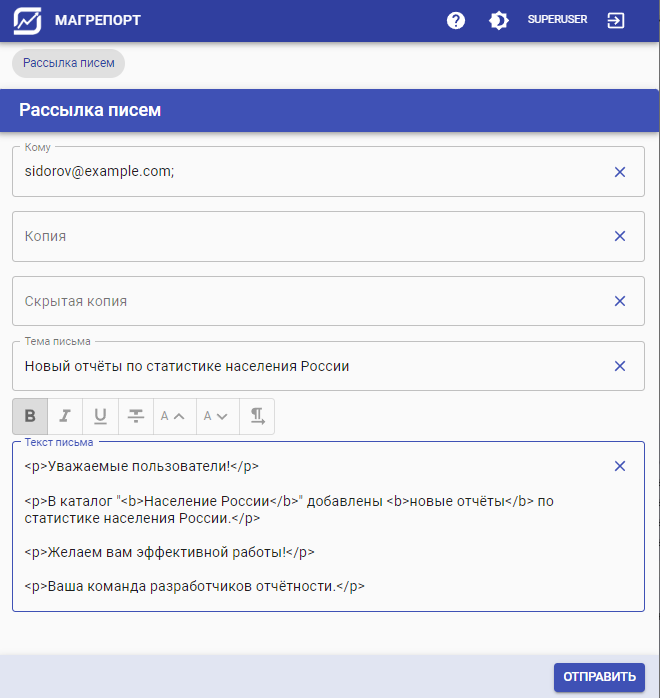
\includegraphics[width=\graphicswidth]{img/27-send-mail-form.png}
		\caption{Форма отправки письма}
		\label{fig:send-mail-form}
	\end{figure}

	При нажатии кнопки <<Отправить>> открывается окно предварительного просмотра, в котором указано количество получателей и привдено само сообщение в отформатированном виде (см. рис. \ref{fig:send-mail-form}). Из данного окна можно отправить письмо, либо вернуться к редактированию его содержания.
	
	\begin{figure}[h]
		\centering
		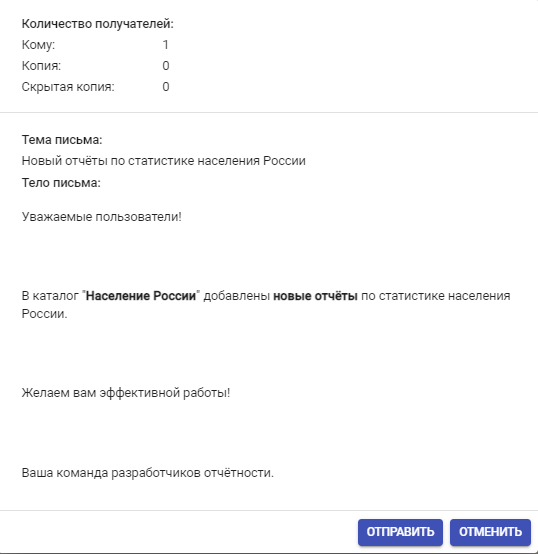
\includegraphics[width=\graphicswidth]{img/28-send-mail-preview.png}
		\caption{Окно предварительного просмотра отправляемого письма}
		\label{fig:send-mail-preview}
	\end{figure}
	
	\section{Управление расписаниями}
	
	Для выполнения отчётов по расписанию создаются объекты, называемые расписаниями --- эти объекты определяют конкретное расписание, по которому выполняются отчёты. Расписания создаются в подразделе <<Расписания>> раздела <<Расписание>> бокового меню. Для вызова мастера создания расписания, как обычно, нужно нажать кнопку <<Плюс>> в правом нижнем углу экрана и выбрать единственный доступный пункт <<Добавить расписание>>. Расписания не упорядочиваются по каталогам.
	
	При создании и редактировании расписания указываются, как и для каждого другого объекта, название и описание. Затем указывается тип расписания и в зависимости от выбранного типа расписания указываются дополнительные параметры расписания (см. рис. \ref{fig:schedule-create}). Существуют следующие типы расписания:
	
	
	\begin{itemize}
		\item \textit{Каждый день в заданное время} --- выполняется каждый день в заданное время.
		
		\item \textit{По указанному дню недели в заданное время} --- выполняется каждый указанный день недели (понедельник, вторник, ..., воскресенье) в указанное время.
		
		\item По указанному дню месяца в заданное время --- выполняется каждый указанный день месяца (1, 2, 3, ..., 31) в указанное время. Если в месяце нет дня с таким номером --- расписание не срабатывает и никуда не переносится.
		
		\item По указанному дню до конца месяца --- выполняется каждый указанный день (1, 2, 3, ..., 31), считая от последнего дня месяца к первому, в указанное время. То есть 1 - последний день месяца, 2 - предпоследний и т.д. Если в месяце нет указанного дня --- расписание не срабатывает и никуда не переносится. 
		
		\item По дню недели с соответствующим порядковым номером от начала месяца в заданное время --- выполняется по указанным дням недели (понедельник, вторник, ..., воскресенье), имеющим указанный порядковый номер от начала месяца (1, 2, ... 5) в указанное время. То есть, например, первый понедельник месяца, вторая пятница месяца и т.п. Если в месяце нет соответствующего дня --- расписание не срабатывает и никуда не переносится.
		
		\item По дню недели с соответствующим порядковым номером от конца месяца в заданное время --- выполняется по указанным дням недели (понедельник, вторник, ..., воскресенье), имеющим указанный порядковый номер от конца месяца (1, 2, ... 5) в указанное время. То есть, например, последний четверг месяца (порядкоый номер --- 1), предпоследняя среда месяца (порядковый номер --- 2) и т.п. Если в месяце нет соответствующего дня --- расписание не срабатывает и никуда не переносится.
		
		\item По требованию --- тригером выполнения отчётов на таком расписании является HTTP-запрос по указанному URL, специфичному для данного отчёта на этом расписании. Само по себе это расписание не имеет такого URL, поэтому не имеет смысла создавать несколько расписаний данного типа.
		
	\end{itemize}

	\begin{figure}[h]
		\centering
		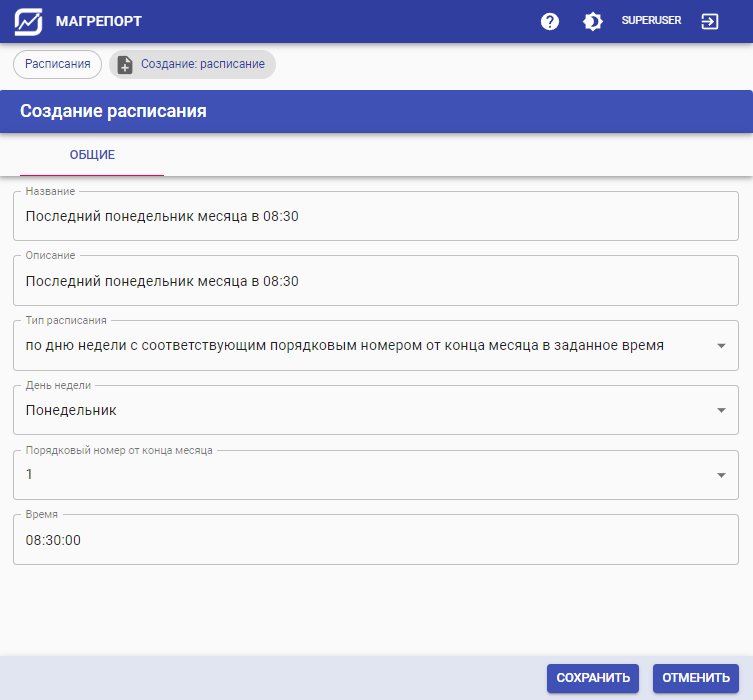
\includegraphics[width=\graphicswidth]{img/29-schedule-create.png}
		\caption{Мастер создания объекта расписания}
		\label{fig:schedule-create}
	\end{figure}
	
	\section{Управление рассылками отчётов по расписанию} \label{administration:schedule-reports}
	
	Магрепорт может выполнять отчёты по заданному расписанию и/или по событию. Выполненный отчёт может быть либо отправлен в виде файла Excel по электронной почте пользователю, либо (если его размер слишком велик) отправлен в виде ссылки на скачиваение файла Excel по электронной почте пользователю, либо предоставлен пользователю в виде задания, к которому пользователь получает доступ. Для того, чтобы установить отчёт на выполнение по расписанию, необходимо в подразделе <<Отчёты на расписании>> раздела <<Расписание>> бокового меню нажать кнопку <<Плюс>> в правом нижнем углу и выбрать единественный доступный пункт меню <<Добавить отчёт на расписании>>. При постановке отчёта на расписании необходимо:
	
	\begin{itemize}
		\item На вкладке <<Общие>> (см. рис. \ref{fig:schedule-report-create-1}) выбрать отчёт, который ставится на расписание, указать название и описание создаваемого объекта и выбрать шаблон Excel, в который будет выгружен отчёт (для отчётов, добавляемых в задания, это не имеет значения, можно оставить шаблон по умолчанию).
		
		\item На вкладке <<Расписания>> (см. рис. \ref{fig:schedule-report-create-2}) выбрать одно или несколько расписаний и указать срок окончания действия рассылки. В Магрепорт рассылки не могут быть бессрочными. Максимальный срок на который создаётся рассылка --- полгода. При приближении к дате истечения рассылки (см. пункт \ref{subsection:schedule-service-settings}) получателям отчёта отправляется уведомление об истечении срока действия рассылки и ссылка на автоматическое продление рассылки ещё на полгода. При переходе по ссылке осуществляется автоматическое продление действия рассылки. Если среди выбранных расписаний встречается расписание с типом <<По требованию>>, появляется поле <<Ссылка для запуска по коду>> с указанием ссылки на тригер события выполнения отчёта и рассылки. Ссылка содержит в себе код, который генерируется автоматически и должен быть уникальным для каждой рассылки. При нарушении уникальности сервер не даст сохранить рассылку --- нужно будет изменить код. Возможности инициировать одним обращением по URL выполнение нескольких рассылок нет.
		
		\item На вкладке <<Рассылка>> (см. рис. \ref{fig:schedule-report-create-3}) задаётся информация о получателях отчёта и способе доставки выполненного отчёта. В поле <<Тип рассылки>> указывается тип <<E-mail>> для рассылки по электронной почте и <<Задания>> для добавления выполненного отчёта в задания пользователя. В случае выбора типа <<E-mail>> файл отчёта либо приходит непосредственно в письме (если его размер меньше 11 млн. байт), либо отправляется в виде ссылки на скачивание файла с сервера. В качестве получателей письма (то есть если тип <<E-mail>>) можно указать как конкретные почтовые адреса (в поле <<Адреса>>), так и выбрать пользоваталей Магрепорт или роли Магрепорт - в последнем случае отчёт отправляет всем пользователям с данной ролью. Если есть ограничения на домены, на которые разрешена отправка писем (см. пункт \ref{subsection:email-settings}), отправка не будет осуществляться на адреса, не соответствующие этим ограничениям. При отправке пользователям Магрепорт, отправка осуществляется только пользователям, у которых задан почтовый адрес (импортируется из LDAP). Если тема или тело письма оставлены пустыми, вместо них подставляется значение из шаблона соответствующего письма (см. раздел \ref{section:letters-templates}). Если пустой отчёт не требуется отправлять, необходимо снять галочку с поля <<Отправлять пустой отчёт?>>. Для типа рассылки <<Задание>> указываются только пользователи и/или роли Магрепорт в качестве получателей.
		
		\item На вкладке <<Падение рассылки>> (см. рис. \ref{fig:schedule-report-create-4}) можно задать пераметры отправки сообщения об ошибке выполнения отчёта и поведение рассылки при возникновении ошибок. Получатели, тема и тело письма задаются полностью аналогично параметрам отправки письма с отчётом, описанным выше. В поле <<Количество падений>> указывается количество падений выполнения отчёта, после которого рассылка становится неактивной. Если значение равно 0 --- рассылка остаётся активной после любого количества падений. При просмотре или редактировании рассылки в поле <<Количество фактических падений>> отображаеется значение счётчика падений --- сколько падений подряд произошло. Рассылку в неактивном статусе можно активировать при помощи кнопки активации (см. рис. \ref{fig:schedule-report-card}).
		
		\item На вкладке <<Фильтры>> (см. рис. \ref{fig:schedule-report-create-5}) необходимо задать значения фильтров при выполнении отчёта. Если фильтры в отчёте отсутствуют --- вкладка также отсутствует. Если в отчёте присутствуют обязательные фильтры, они должны быть заполнены --- иначе объект рассылки нельзя будет сохранить. Если в отчёте изменён состав фильтров, рассылка становится неактивной, о чём приходит соответствующее почтовое уведомление (см. раздел \ref{section:letters-templates}). В этом случае на карточке отсутвует кнопка активации рассылки --- необходимо зайти в редактирование рассылки, указать правильные значения фильтров и сохранить рассылку.
		
	\end{itemize}

	\begin{figure}[h]
		\centering
		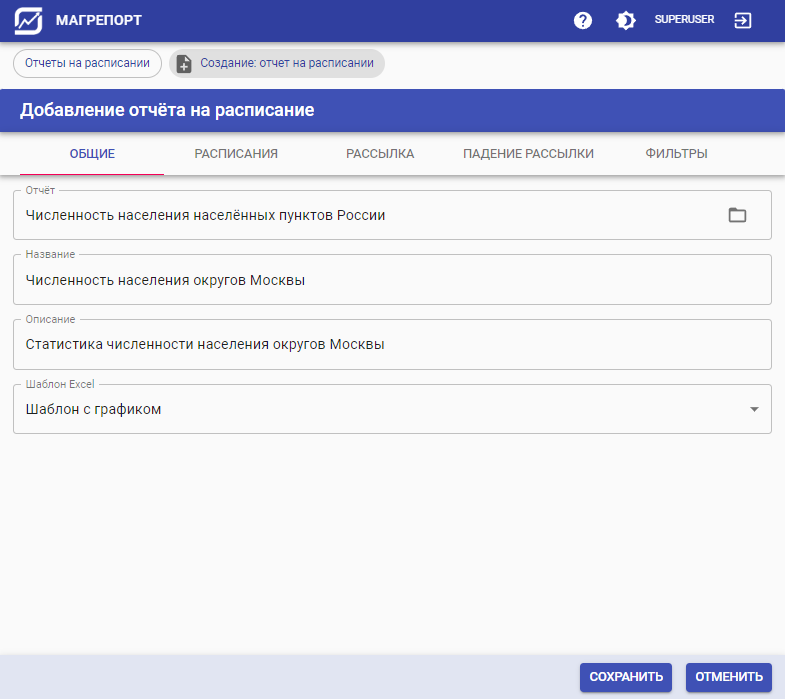
\includegraphics[width=0.47\textwidth]{img/30-schedule-report-create-1.png}
		\caption{Постановка отчёта на расписание - вкладка <<Общие>>}
		\label{fig:schedule-report-create-1}
	\end{figure}


	\begin{figure}[h]
		\centering
		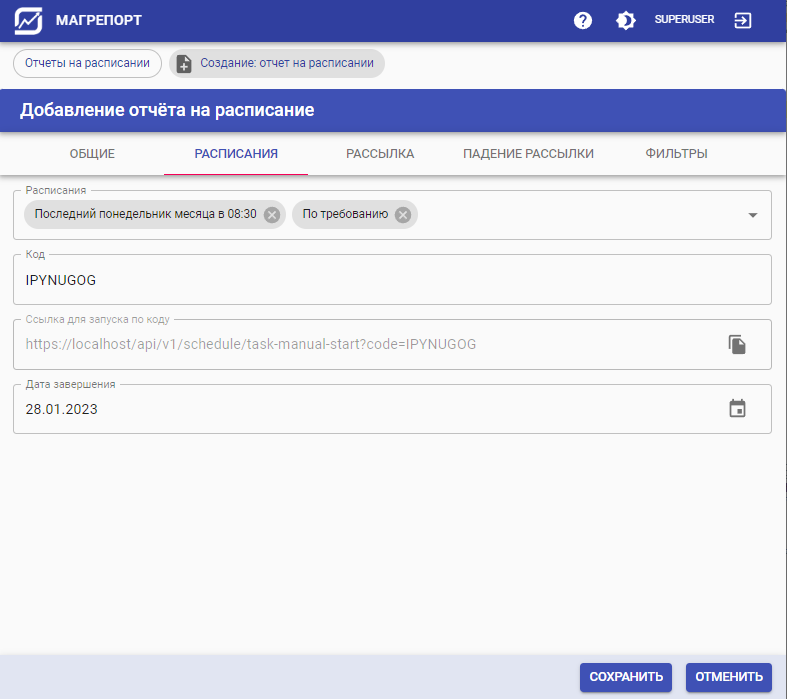
\includegraphics[width=0.47\textwidth]{img/31-schedule-report-create-2.png}
		\caption{Постановка отчёта на расписание - вкладка <<Расписания>>}
		\label{fig:schedule-report-create-2}
	\end{figure}

	\begin{figure}[h]
		\centering
		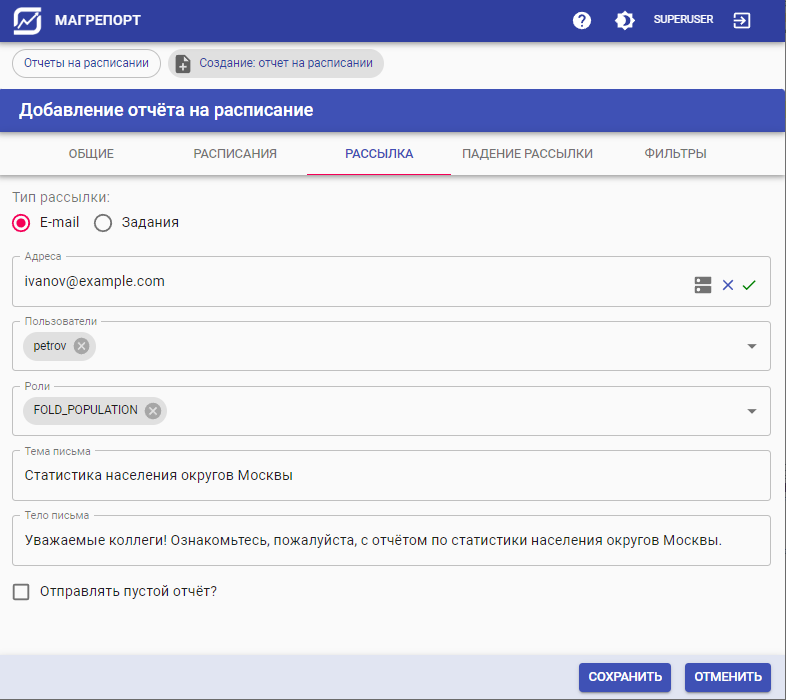
\includegraphics[width=0.47\textwidth]{img/32-schedule-report-create-3.png}
		\caption{Постановка отчёта на расписание - вкладка <<Рассылка>>}
		\label{fig:schedule-report-create-3}
	\end{figure}

	\begin{figure}[h]
		\centering
		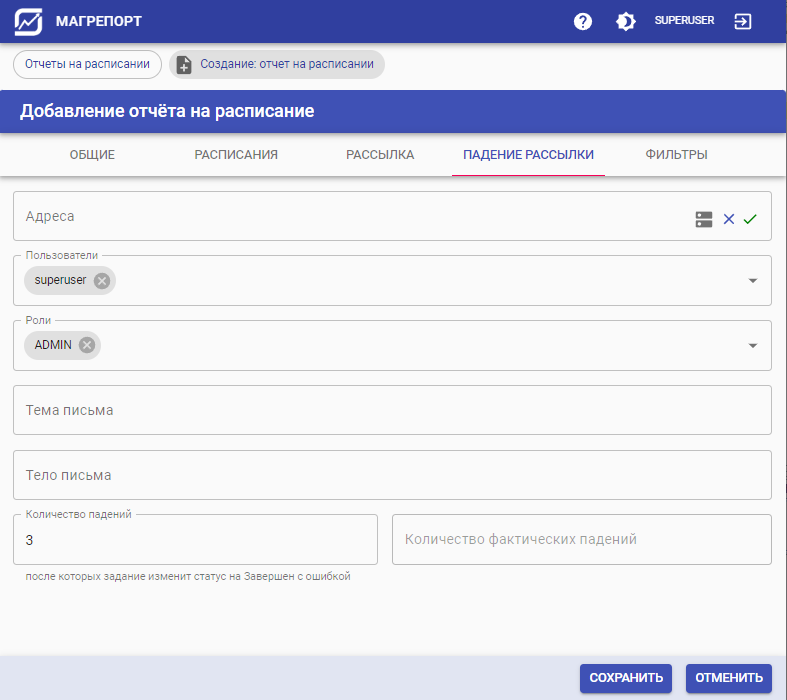
\includegraphics[width=0.47\textwidth]{img/33-schedule-report-create-4.png}
		\caption{Постановка отчёта на расписание - вкладка <<Падение рассылки>>}
		\label{fig:schedule-report-create-4}
	\end{figure}

	\begin{figure}[h]
		\centering
		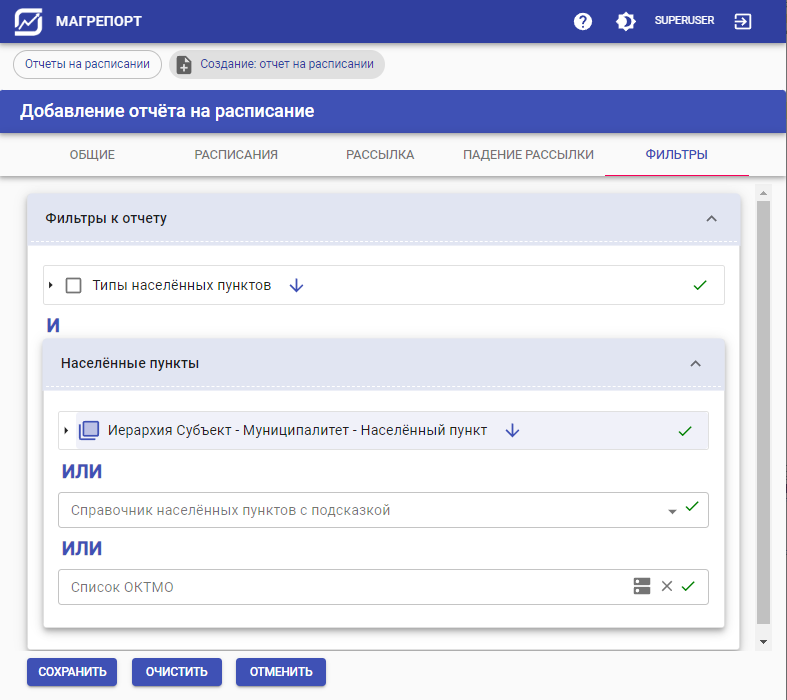
\includegraphics[width=0.47\textwidth]{img/34-schedule-report-create-5.png}
		\caption{Постановка отчёта на расписание - вкладка <<Фильтры>>}
		\label{fig:schedule-report-create-5}
	\end{figure}

	На карточке рассылки (см. рис. \ref{fig:schedule-report-card}) расположена информация об этой рассылке. Непосредственно под названием рассылки расположен статус активности рассылки (в соответствии со статусом происходит цветовое выделение названия рассылки, статуса и панели кнопок рассылки):
	
	\begin{itemize}
		\item \textit{Ожидает выполнения} --- рассылка активна и ожидает очередного своего выполнения по расписанию
		
		\item \textit{Выполняется} --- отчёт на расписании в настоящий момент выполняется
		
		\item \textit{Успешно выполнен} --- отчёт на расписании успешно выполнен и происходит рассылка результатов
		
		\item \textit{Завершен с ошибкой} --- отчёт завершён с ошибкой максимально допустимое количество раз поряд и рассылка не активна
		
		\item \textit{Просрочен срок действия} --- истёк срок действия рассылки, рассылка не активна
		
		\item \textit{Изменены параметры отчета} --- изменены фильтры отчёта, требуется корректировка значений фильтров в рассылке, рассылка не активна
		
		\item \textit{Не активен} --- рассылка неактивна в результате ручного изменения статуса
	\end{itemize}
	
	
	Внизу карточки расположена панель кнопок действий с рассылкой:
	
	\begin{itemize}
		\item \textit{Редактировать} --- редактировать параметры рассылки
		
		\item \textit{Изменить статус} --- выполнить отчёт и рассылку
		
		\item \textit{Изменить статус} --- переключает рассылку между статусами <<Ожидает выполнения>> и <<Неактивен>>, а также возвращает в статус <<Ожидает выполнения>> рассылки со статусом <<Завершен с ошибкой>>
		
		\item \textit{Удалить} --- удаляет рассылку
	\end{itemize}
	
	\begin{figure}[h]
		\centering
		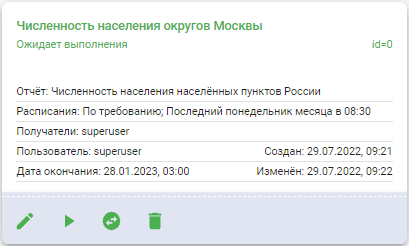
\includegraphics[width=0.47\textwidth]{img/35-schedule-report-card.png}
		\caption{Карточка рассылки}
		\label{fig:schedule-report-card}
	\end{figure}
	
\end{document}